% ===============================
% Data processing
% ===============================
\newpage
\section{Data Processing}
\label{sec:dataproc}

This section is aimed at readers interested in the data processing and display scripts. It details the computational methods used to generate data. Although the chapter clarifies underlying concepts, basic knowledge in how software code is written is helpful to understand it. 

Figure \ref{fig:app_design_perl} shows an overview of the different parts to import and analyze the data. The \ac{perl} scripts that read/write to the database constitute the main part of the
data processing framework (relevant files are listed in Appendix \ref{tab:directories_and_files_overview} on page \pageref{tab:directories_and_files_overview}). 

Figure \ref{fig:app_design_perl} shows an overview of the different parts to import and analyze the data. The \ac{perl} scripts that read/write to the database constitute the main part of the
data processing framework (relevant files are listed in Appendix \ref{tab:directories_and_files_overview} on page \pageref{tab:directories_and_files_overview}). 

\begin{figure}[htpb]
\begin{center}
  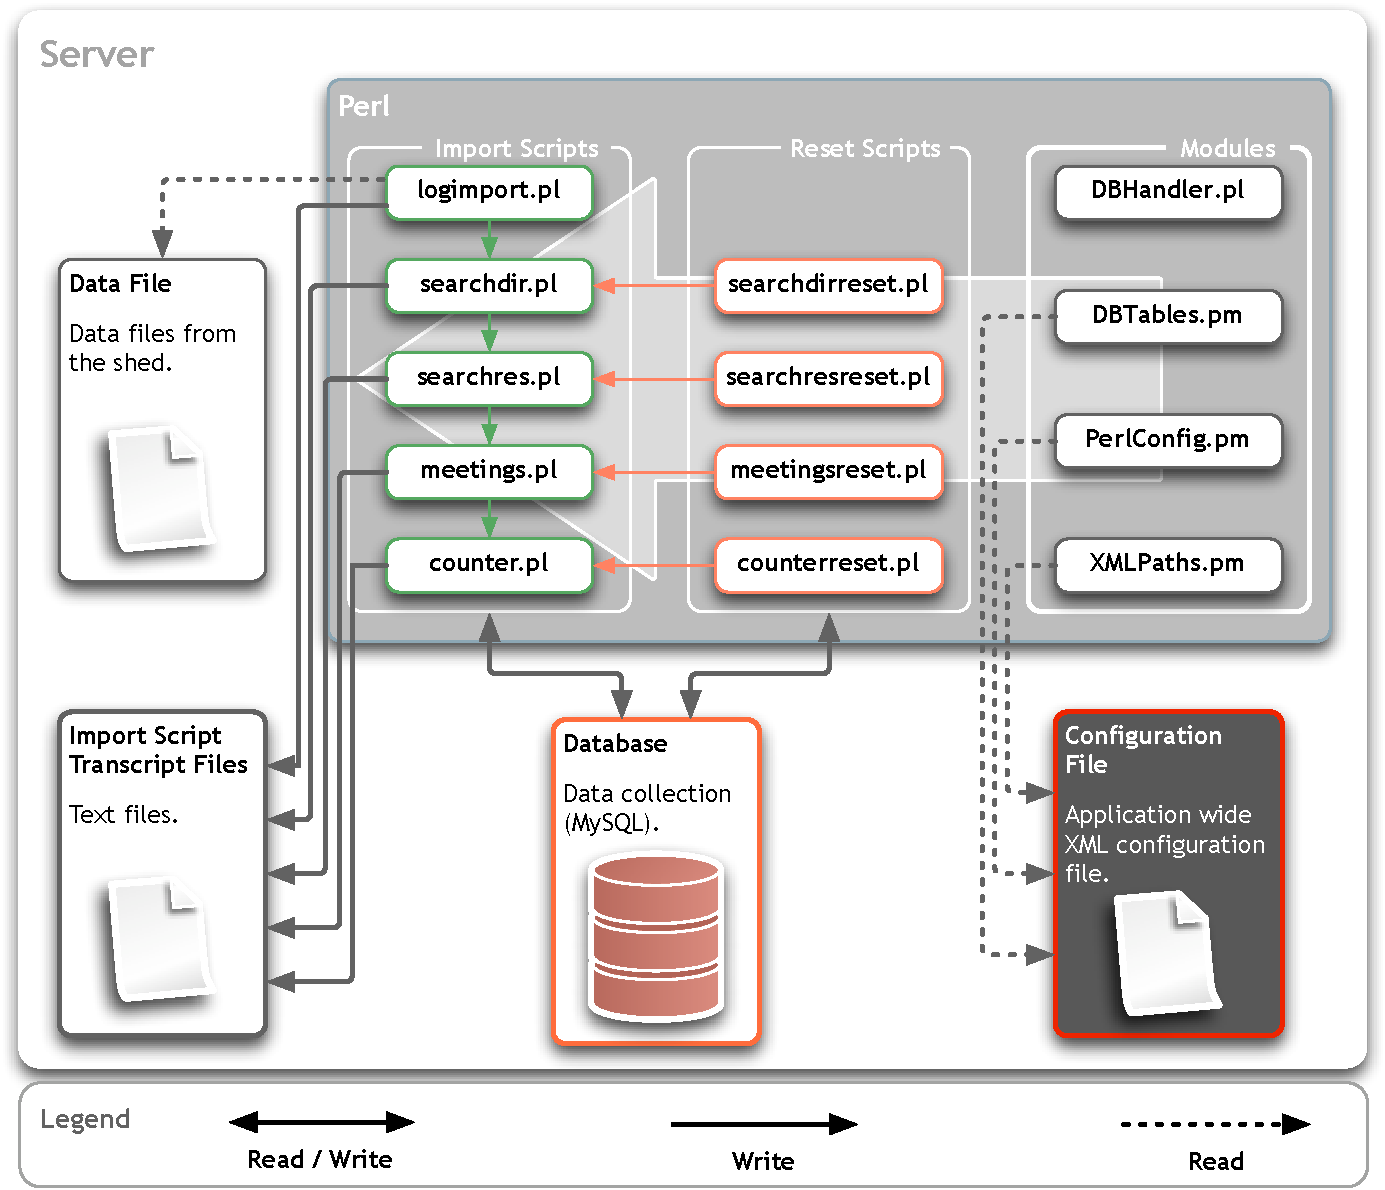
\includegraphics[width=\textwidth]{assets/pdf/app_design_perl.pdf}
  \caption[Schema of data processing]{Schema of the different software parts involved in the data processing.}
  \label{fig:app_design_perl}
\end{center}
\end{figure}

The \textit{Import Scripts} run in a cascade, beginning with the \lstinline|logimport.pl| script, which reads the data files from the barn and ends with the \lstinline|counter.pl| script (indicated in figure \ref{fig:app_design_perl} by the green arrows). Each script writes a transcript file to trace progress. Upon completion of the cascade, data is stored in the respective tables.

A scheduled daily task checks for new data files uploaded to the server and starts the cascade when needed (details in Appendix \ref{app:import_schedule} on page \pageref{app:import_schedule}). 

The \textit{Reset Scripts} set the database back to a state where the import cascade can be rerun, starting with the corresponding import script (indicated in figure \ref{fig:app_design_perl} by the orange arrows). If, for example, the \lstinline|searchdirreset.pl| is executed, the import cascade will be started with the \lstinline|searchdir.pl| script. It is recommended to start the import cascade using the import scripts programmed in BASH language (see Appendix \ref{app:import_schedule} for details).

The \textit{Modules} read out the configuration from the central \ac{XML} based configuration file (see Appendix \ref{app:configperl} for details) and make it available to the import and reset scripts (indicated in figure \ref{fig:app_design_perl} by the large grey arrow with the white border). As the perl scripts interact with the database, the database configuration is read out as well by some of the \textit{Modules} (see Appendix \ref{app:configdb} for details). 

The following sections provide details about each script in the import cascade.

\subsection{Importing}
\label{subsec:importing}

The \lstinline|logimport.pl| extracts the spatial position data from the data files and writes it to the \lstinline|data| table (see \ref{para:data_table} on page \pageref{para:data_table} for the table structure).

Prior to data extraction, the  script creates a backup of the actual database (see Appendix \ref{app:configperl} for details). Subsequently, the data is extracted from the data files and written to the database. 

As mentioned in section \ref{subsec:problems}, some of the antennas could not be addressed properly. Therefore, the script has to catch these exceptional values and convert them to the designated ones (see Appendix \ref{app:antenna_adress_conversions} for the list of conversions).

\subsection{Direction results}
\label{subsec:dirres}

The \lstinline|searchdir.pl| script searches for matching pairs of antenna readings in the \lstinline|data| table, which serves to build a \textit{direction result}. A pair matches if:

\begin{mylist}
\item The RFID of both readings is the same,
\item The time difference (in seconds) between the two readings is not greater than the value set as the \lstinline|<antennaInterval>| value in the configuration file (see Appendix \ref{app:configperl} for details), 
\item The readings originate from both antennas attached to a box.
\end{mylist}

Figure \ref{fig:direction_result} shows the composition of a direction \textit{in} and a direction \textit{out} by means of an example at nestbox 16. The \lstinline|<antennaInterval>| value is set to 5 seconds. Although, the interval value has been estimated at first, it could be justified afterwards. Figure \ref{fig:dist_dir_elapse} shows the distribution of elapsed milliseconds between the two antenna readings, separated by direction. Based on this distribution, the interval value could even be reduced.
 
\begin{figure}[htpb]
\begin{center}
  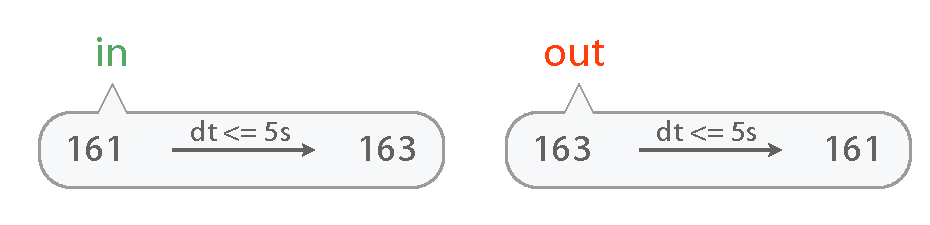
\includegraphics[width=0.75\textwidth]{assets/pdf/direction_result_schema.pdf}
  \caption[Illustration of a direction result]{Illustration of the possible composition of a \textit{direction result}.}
  \label{fig:direction_result}
\end{center}
\end{figure}

\begin{figure}[htpb]% 
\centering 
\subfloat[][]{
\label{fig:dirin_ant_read_distr} %
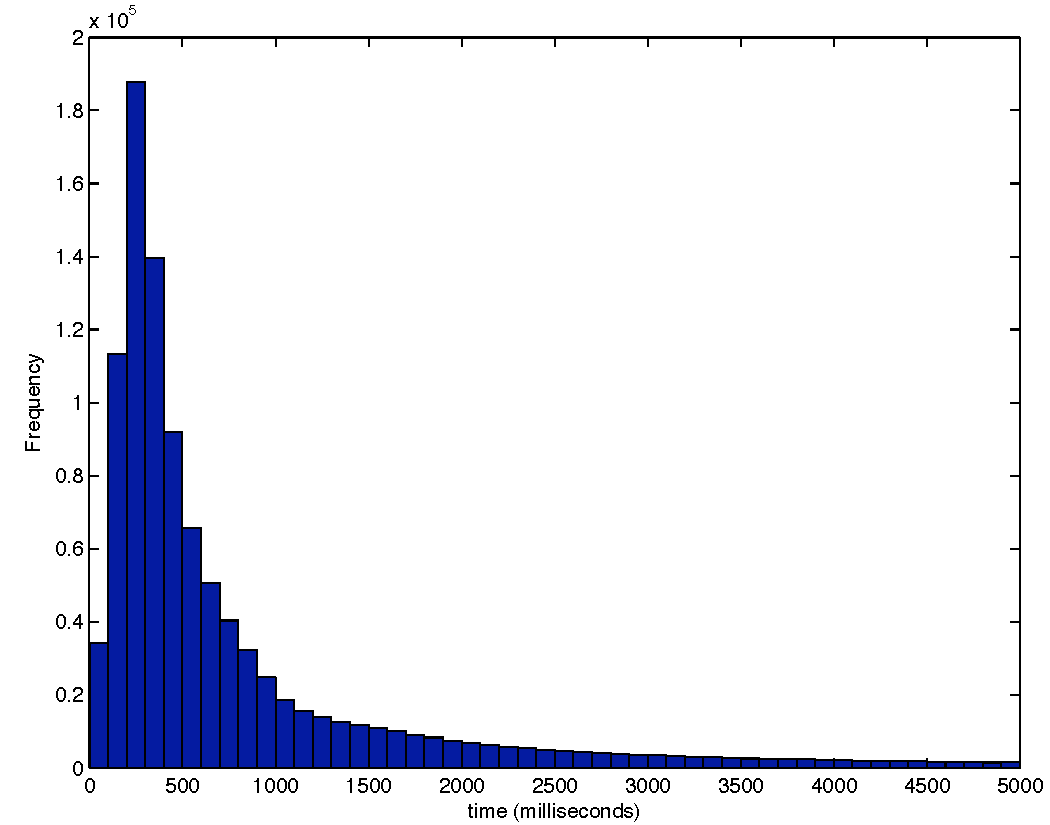
\includegraphics[width=.45\textwidth]{assets/pdf/dirin_ant_read_distr.pdf}
}% 
\qquad 
\subfloat[][]{
\label{fig:dirout_ant_read_distr}%
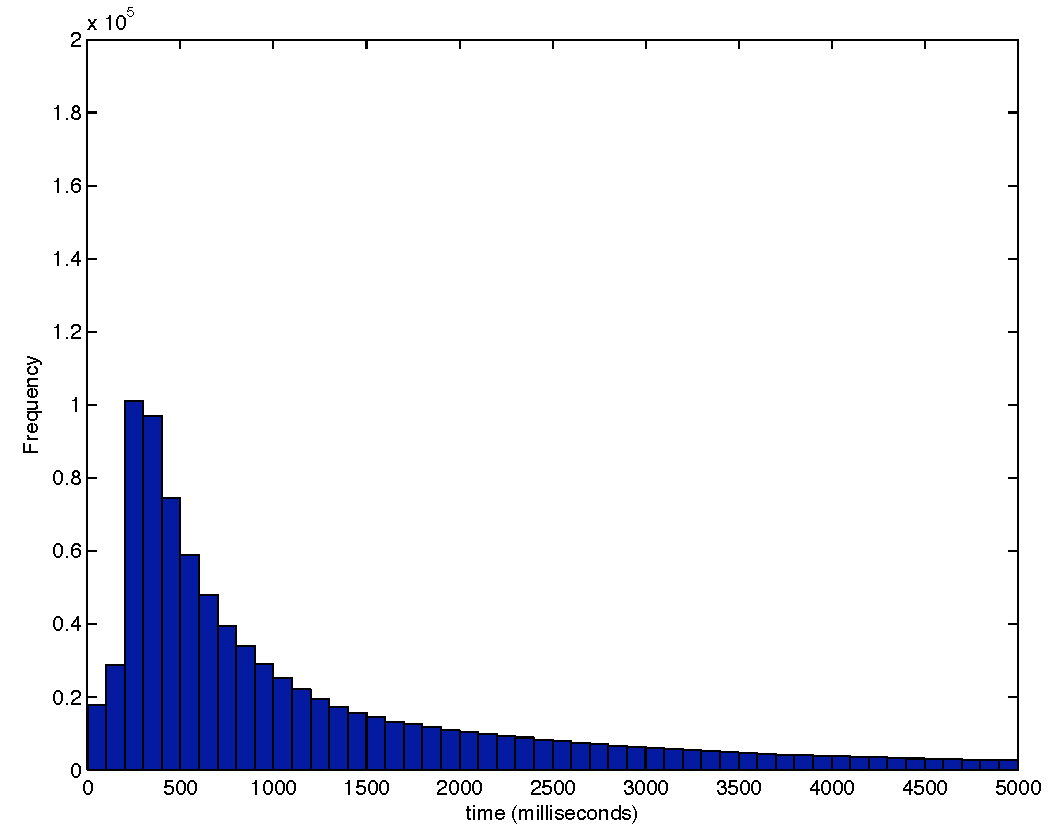
\includegraphics[width=.45\textwidth]{assets/pdf/dirout_ant_read_distr.pdf}
} 
\caption[Frequencies of elapsed time between antenna readings of direction results]{Frequencies of elapsed time between two antenna readings for \lstinline|direction results| with direction \lstinline|in| \subref{fig:dirin_ant_read_distr} and direction \lstinline|out| \subref{fig:dirout_ant_read_distr}. \footnotesize(Charts courtesy of Nicolas Perony.)}
\label{fig:dist_dir_elapse} 

\end{figure}

The findings are written to the \lstinline|dir| table (see section \ref{para:dir_table} on page \pageref{para:dir_table} for the table structure). The value for the \lstinline|time| field of the \textit{direction result} is always set to the time value of the reading at the outer antenna. Therefore, a mouse is said to have left a box when it passes the outer antenna.

If the \lstinline|<antennaInterval>| is changed, the \lstinline| searchdirreset.pl| must be executed and followed by the scripts in the import cascade starting with the \lstinline|searchdir.pl| script. 

\subsection{Stay results}
\label{subsec:stayres}

The \lstinline|searchres.pl| aims to find matching \textit{direction results} in the \lstinline|dir| table, which build a \textit{stay result}.

A pair of \textit{direction results} matches if the following 3 conditions are satisfied:

\begin{mylist}
\item RFIDS's of both \textit{direction results} are the same,
\item \textit{direction results} have opposite \lstinline|direction| values,
\item \textit{direction results} are recorded at the same nestbox.
\end{mylist}

A \textit{stay result} is found as well, if a \textit{direction result} can be paired with an unused dataset (i.e. a dataset which is not used in a \lstinline|direction result|). 

Such a pair matches if the following conditions are satisfied:
 
\begin{mylist}
	\item The RFIDS's of the \textit{direction result} and the unused dataset are the same,
	\item The \textit{direction result} has a \lstinline|dir| value of \lstinline|in| (i.e. the mouse enters the nestbox),
	\item The unused dataset is recorded at the outer antenna of the nestbox (i.e. the mouse leaves the nestbox),
	\item The \textit{direction result} and the unused dataset are recorded at the same nestbox.  
\end{mylist}

In the former case, the \textit{stay result} is of \textbf{type 3}, in the latter case as of \textbf{type 4}. Figures \ref{fig:type_3_stay_result} and \ref{fig:type_4_stay_result} illustrate the differences between the types by means of an example at box 16. The \lstinline|<antennaInterval>| value is set to 5 seconds. Of the \textit{stay results} currently in the database, 85.8\% are type 3 results and 14.2\% type 4. 

\begin{figure}[htpb]
\begin{center}
  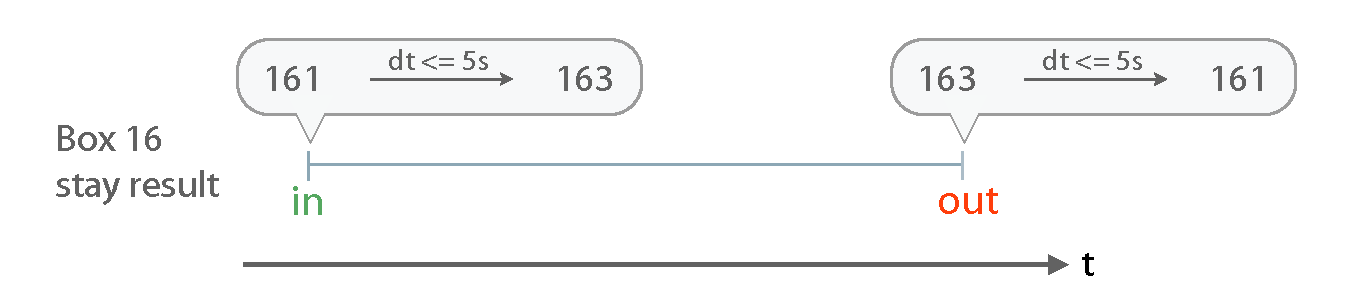
\includegraphics[width=0.75\textwidth]{assets/pdf/stay_result_type_3_schema.pdf}
  \caption[Illustration of a type 3 \textit{stay result}]{Illustration of a Type 3 \textit{stay result} at box 16,  made of \lstinline|in| and \lstinline|out| direction results.}
  \label{fig:type_3_stay_result}
\end{center}
\end{figure}

\begin{figure}[htpb]
\begin{center}
  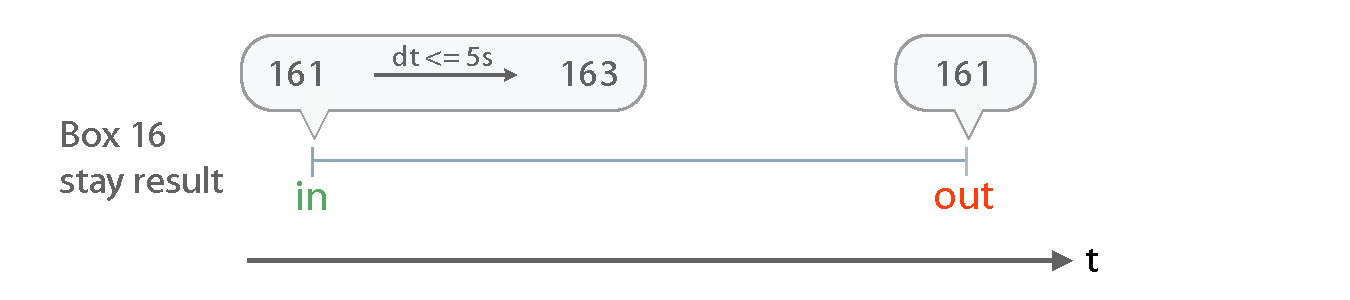
\includegraphics[width=0.75\textwidth]{assets/pdf/stay_result_type_4_schema.pdf}
  \caption[Illustration of a type 4 \textit{stay result}]{Illustration of a Type 4 \textit{stay result} made up of an \lstinline|in| direction result and a reading at the outer antenna.}
  \label{fig:type_4_stay_result}
\end{center}
\end{figure}

Additionally, the script handles the temporal overlaps within the \textit{stay results}. As explained in section \ref{subsec:problems}, the overlaps occur because the antenna system is imperfect. If the script kept all possible \textit{stay results}, situations illustrated in figures \ref{fig:result_overlap} and \ref{fig:result_overlap_single} would arise. All the \textit{stay results} (1, 2, and 3) originate from the same transponder recorded at the same or other nestboxes. Hence, the antenna system must have missed readings, but we have no clue about the exact moment.  

Illustrated in figure \ref{fig:result_overlap} is the situation where one \textit{stay result} (1) overlaps two others (2),(3). A reasonable explanation is that there are several antenna recordings missing. Since we have two \textit{stay results}, (2) and (3), which look valid, we discard \textit{stay result} (1) where we don't know what really happened. Furthermore, this approach is reasonable as the probability of missed antenna readings is much higher than the probability that eight antenna readings (two per \textit{direction result}) that constitute two perfect-looking \textit{stay results} are wrong.

\begin{figure}[htpb]
\begin{center}
  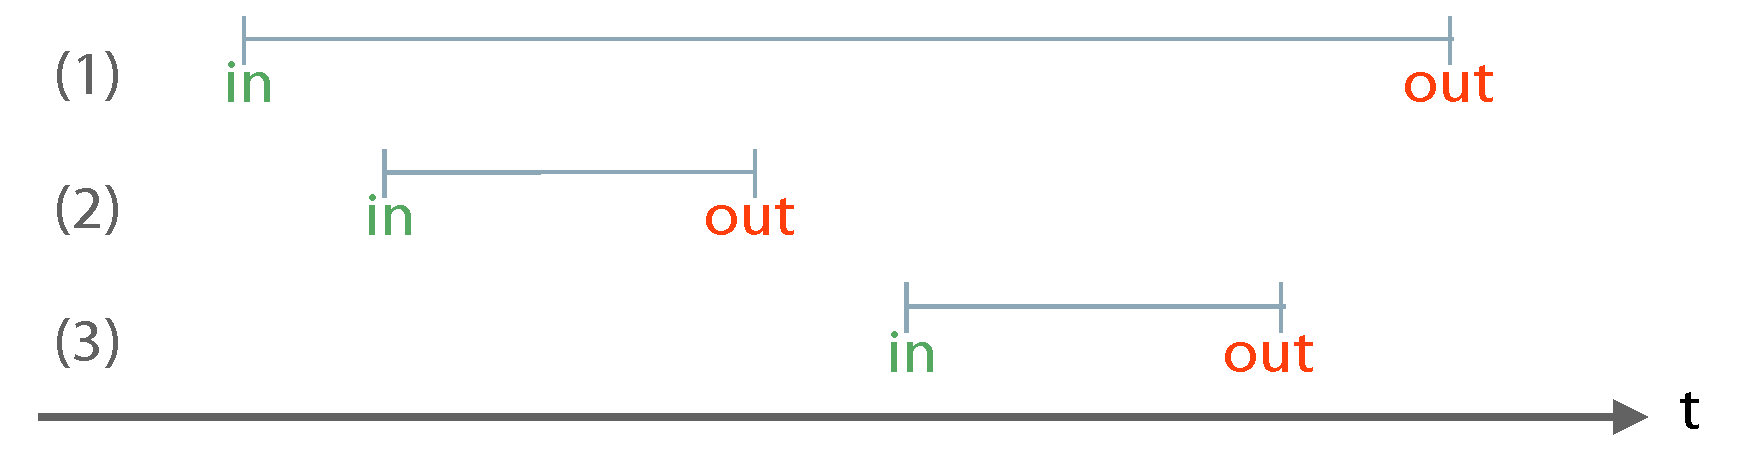
\includegraphics[width=0.75\textwidth]{assets/pdf/result_overlaps_schema.pdf}
  \caption[Illustration of a possible result overlap situation]{Illustration of a possible result overlap situation, where a \textit{stay result} overlaps many others.}
  \label{fig:result_overlap}
\end{center}
\end{figure}

Figures \ref{fig:result_overlap_single} and \ref{fig:result_overlap_single_shifted} illustrate the situation where one \textit{stay result} overlaps another. In this case, the \textit{stay result} (1) is discarded as well.

The justification for this approach is similar to the one just discussed: \textit{Stay result} (2) looks valid, but there must be missed antenna readings. In figure \ref{fig:result_overlap_single_shifted}, the two \textit{stay results} are only partly overlapping. \textit{Stay result} (1) is discarded as well, but \textit{stay result} (2) will be discarded in the next step to eliminate temporal overlaps.      

\begin{figure}[htpb]
\begin{center}
  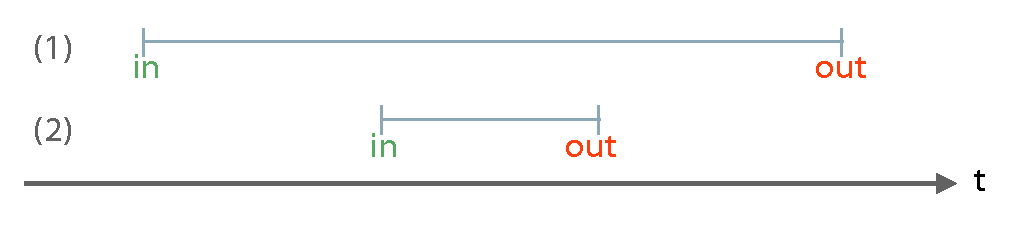
\includegraphics[width=0.75\textwidth]{assets/pdf/result_overlaps_single_schema.pdf}
  \caption[Single result full overlap situation]{Illustration of a possible result overlap situation where a \textit{stay result} fully overlaps another.}
  \label{fig:result_overlap_single}
\end{center}
\end{figure} 

\begin{figure}[htpb]
\begin{center}
  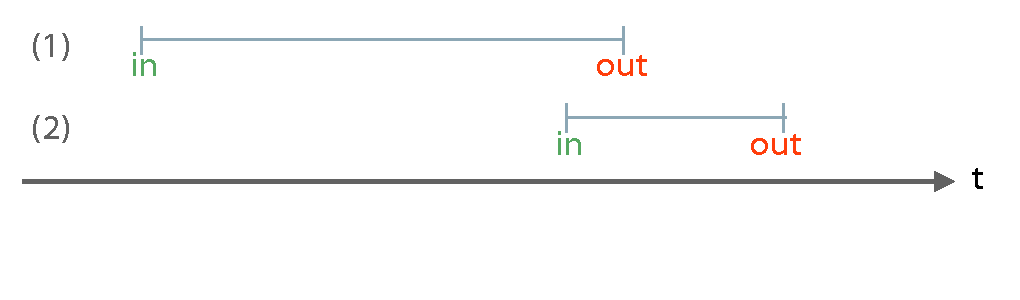
\includegraphics[width=0.75\textwidth]{assets/pdf/result_overlaps_single_shifted_schema.pdf}
  \caption[Single result partly overlapped]{Illustration of a possible result overlap situation where a \textit{stay result} partly overlaps another.}
  \label{fig:result_overlap_single_shifted}
\end{center}
\end{figure}

If the \textit{stay result} does not overlap another the script checks for other antenna readings that were recorded during the \textit{stay result}. This is illustrated in figure \ref{fig:dataset_overlap}. Obviously, only antenna readings which originate from the same transponder are taken into account.

In figure \ref{fig:dataset_overlap} four other antenna readings could be found, two of them happen not to be from the same nestbox. This \textit{stay result} will be discarded, as we don't know what really happened.

\begin{figure}[htpb]
\begin{center}
  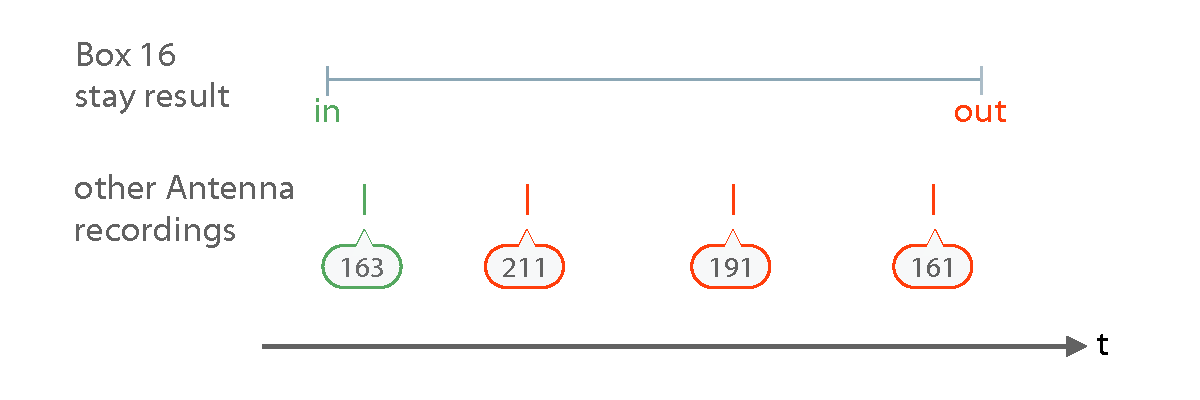
\includegraphics[width=0.75\textwidth]{assets/pdf/dataset_overlap_schema.pdf}
  \caption[Dataset overlapping]{Illustration of a possible dataset overlap situation where other antenna readings have been found during a \textit{stay result}.}
  \label{fig:dataset_overlap}
\end{center}
\end{figure}

As seen in figure \ref{fig:dataset_overlap}, the reading from antenna \lstinline|163| at nestbox 16 is colored green. If we consider the situation illustrated in figure \ref{fig:dataset_overlap_nervous}, we can see that several datasets which are exclusively recorded at the inner antenna of nestbox 16 are overlapped by the \textit{stay result}. In such a case we keep the result, as the mouse has not left the box and might only be nervously inspecting the entry tube. As stated in section \ref{subsec:dirres}, a mouse is out of the box if it is recorded at the outer antenna. 

The \textit{nervous index} is the number of readings at the inner antenna during the \textit{stay result}. The \textit{nervous index} is 4 for the situation shown in figure \ref{fig:dataset_overlap_nervous}. This value is written to the database as explained in section \ref{para:res_table}.

\begin{figure}[htpb]
\begin{center}
  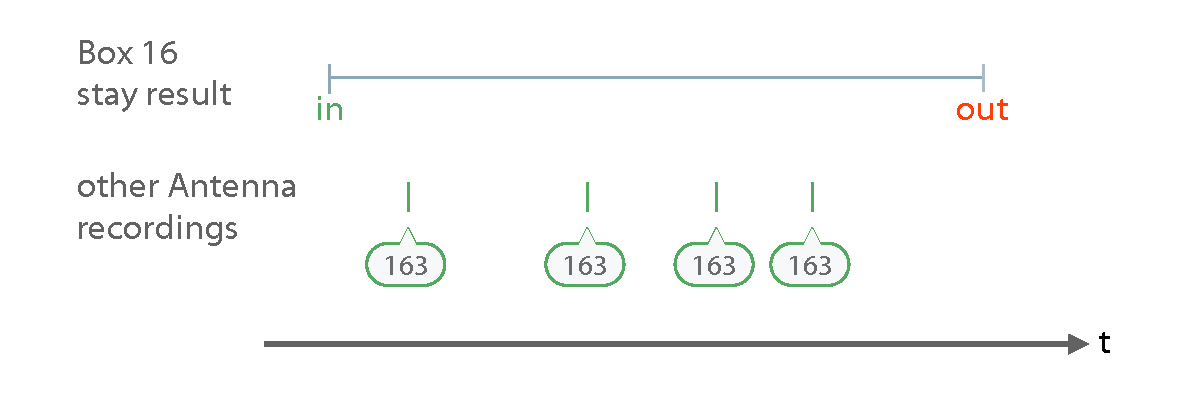
\includegraphics[width=0.75\textwidth]{assets/pdf/dataset_overlap_nervous_schema.pdf}
  \caption[\textit{Nervous mouse}]{Illustration of a possible dataset overlap situation, where other antenna readings have been found during a \textit{stay result}, but exclusively at the box's inner antenna. Such a situation is identified as a \textit{nervous mouse}.}
  \label{fig:dataset_overlap_nervous}
\end{center}
\end{figure}
 
The search for the \textit{stay result} overlaps and the overlapped antenna recordings could be combined. Though, we are interested in the influence of these steps on the numbers. In the period from the 5th of April 2007 to the 27th of March 2009, 1.5 million \textit{direction results} with a direction value of \lstinline|in| are found. Without any overlap filtering, the script finds a \textit{stay result} for 99.0\% of the direction results. After excluding the \textit{stay result} overlaps, 68.1\% remain, and 66.2\% after excluding the \textit{stay results} with overlapping antenna readings. Though, 59.6\% of the remaining \textit{stay results} are \textit{nervous mouse} results.

Nevertheless, an inconsistency remains. 0.05\% of the \textit{stay result} show a duration of stay longer than nine hours. These values are implausible as the mice have to drink outside the nestbox, for example. However, these results exist in the database and are validated. A number of explanations have been discussed how such results can arise, which are quite complicated and unlikely, but therefore could be true for these exceptional cases. These results may be removed from display (see section \ref{subsec:miceminer_config} on page \pageref{subsec:miceminer_config}) but kept in the database.     

The \textit{stay results} are written to the \lstinline|res| table as described in paragraph \ref{para:res_table} on page \pageref{para:res_table}.

\subsection{Meeting results}
\label{subsec:meetingres}

The \lstinline|meetings.pl| script determines when and how many time the mice spend together in the nestboxes. 

Consider the situation that two \textit{stay results} of different RFID's recorded at the same nestbox temporally overlap. In such a situation, the two mice meet in the nestbox and a \textit{meeting result} is found.

Additionally, the script analyzes how two mice meet. There are four different possibilities, as shown in figure \ref{fig:meeting_types} and explained in the following list:

\begin{mydesc}
\label{list:meeting_types}
\item \textbf{Type 1}: Tr. B entered the nestbox, while Tr. A was already in the box, and Tr. B left the nestbox, while Tr. A was still in the box. 
\item \textbf{Type 2}: Tr. A entered the nestbox, while Tr. B was already in the box, and Tr. A left the nestbox, while Tr. B was still in the box. 
\item \textbf{Type 3}: Tr. A entered the nestbox, while Tr. B was already in the box, and Tr. B left the nestbox, while Tr. A was still in the box. 
\item \textbf{Type 4}: Tr. A entered the nestbox, while Tr. B was already in the box, and Tr. B left the nestbox, while Tr. A was still in the box. 
\end{mydesc}

\begin{figure}[htpb]
\begin{center}
  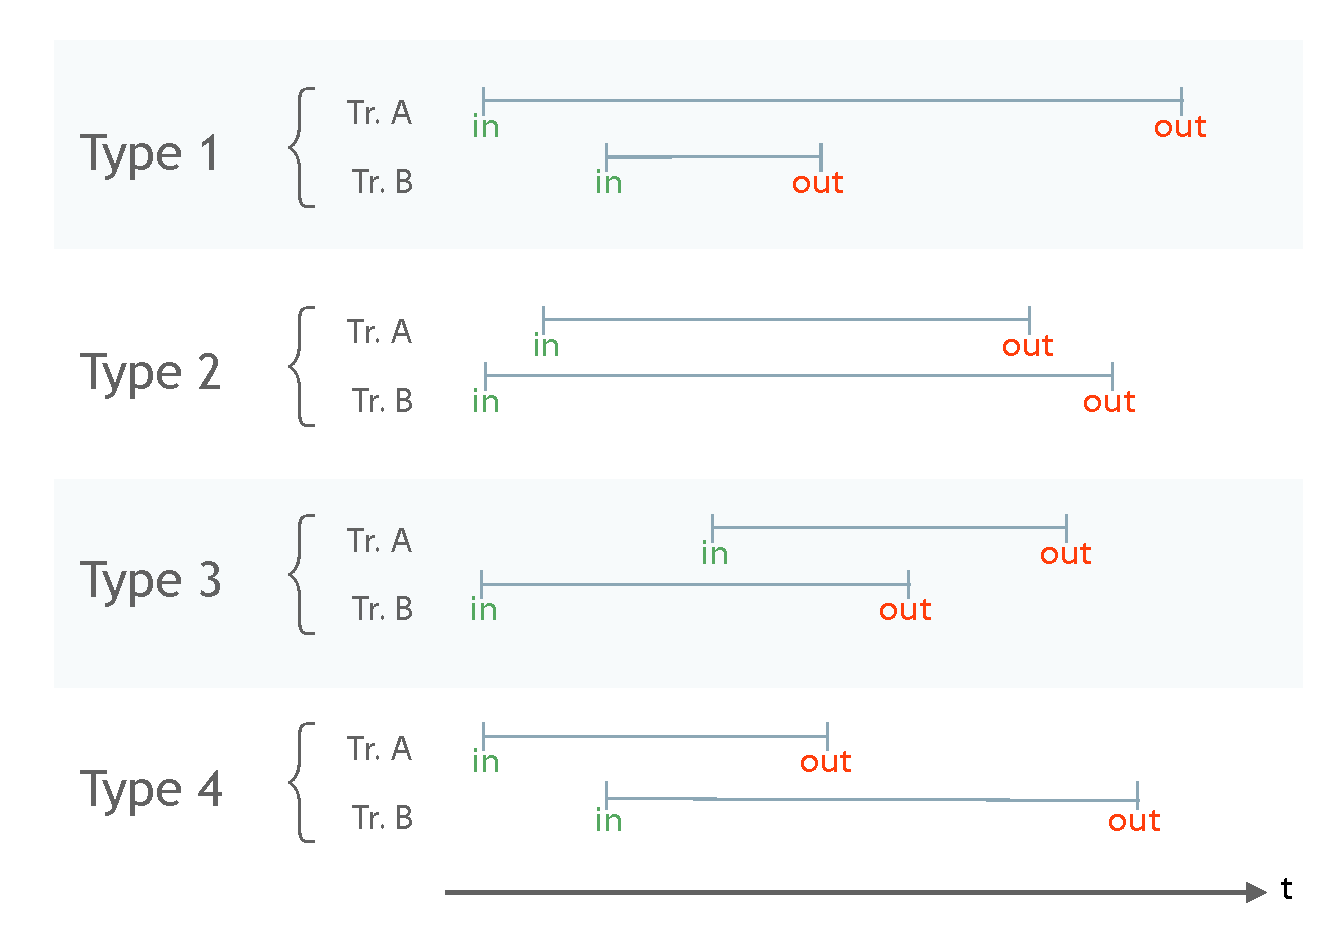
\includegraphics[width=0.66\textwidth]{assets/pdf/meeting_types_schema.pdf}
  \caption[illustration of meeting result types]{Illustration of possible meeting situations in a nestbox with two mice (Tr. A, Tr. B).}
  \label{fig:meeting_types}
\end{center}
\end{figure}

However, the \textit{meeting result} types and explanations above only apply if we look at the situations from the viewpoint of mouse Tr. A. When looking at the situations from Tr. B, the types are swapped as follows:

\begin{mylist}
\item Type 1 is swapped to \textbf{Type 2}   
\item Type 2 is swapped to \textbf{Type 1}
\item Type 3 is swapped to \textbf{Type 4} 
\item Type 4 is swapped to \textbf{Type 3}
\end{mylist}

As mentioned in the section about the \textit{stay results}, a few results show an impractical duration of stay. Since the \textit{meeting results} are derived from the \textit{stay results}, a few impossible \textit{meeting results} (97 or 0.01\%) follow. As for the \lstinline|stay results|, these \textit{meeting results} can be excluded from display in the user interface.

The \textit{meeting results}, are written to the \lstinline|meetings| table as described in paragraph \ref{para:meetings_table} on page \pageref{para:meetings_table}. 

The rules in the data processing were accurately determined based on several cycles of calculation. After each pass, the rules have been adjusted to reduce inconsistencies. In the final procedure presented in this section, inconsistencies are removed without loss of to many results.
